\begin{figure}[t]
\centering
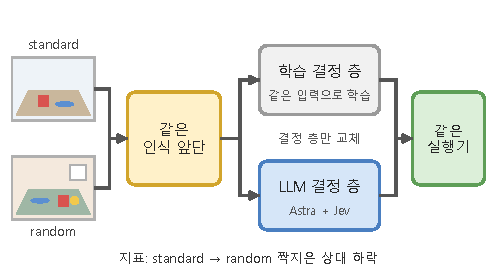
\includegraphics[width=\linewidth]{figures/eval_protocol.pdf}
\caption{\textbf{평가 프로토콜.} 같은 layout의 standard와 random 장면을 짝지어 돌리고 상대 하락(RD)을 잰다. 상위 계획기(Astra, 학습한 8B·35B, 첫 계획 뒤 끔)와 구성(VLA 단독, 상위 단독, 상위 + VLA)을 한 축씩 바꾸고, $\pi_{0.5}$ 미세조정·코드 정책·규칙 기준선을 같은 짝에서 돌린다. 지연 충실 트랙과 동기 공정 트랙을 같은 표에 둔다. 장면 그림은 설명용이다.}
\label{fig:eval}
\end{figure}
